\documentclass{beamer}
\usepackage{amsmath}
\usepackage{amsthm}
\usepackage{amsfonts}
\usepackage{bbm}
\usepackage{ifpdf}
\usepackage{float}
\usepackage{fancyhdr}

\usepackage{subcaption}
\usepackage{afterpage}
\usepackage{rotating}
\usepackage{multirow}



% ignore the follwing script, it fixes a known bug in beamer
\makeatletter
\renewcommand{\itemize}[1][]{%
  \beamer@ifempty{#1}{}{\def\beamer@defaultospec{#1}}%
  \ifnum \@itemdepth >2\relax\@toodeep\else
    \advance\@itemdepth\@ne
    \beamer@computepref\@itemdepth% sets \beameritemnestingprefix
    \usebeamerfont{itemize/enumerate \beameritemnestingprefix body}%
    \usebeamercolor[fg]{itemize/enumerate \beameritemnestingprefix body}%
    \usebeamertemplate{itemize/enumerate \beameritemnestingprefix body begin}%
    \list
      {\usebeamertemplate{itemize \beameritemnestingprefix item}}
      {\def\makelabel##1{%
          {%
            \hss\llap{{%
                \usebeamerfont*{itemize \beameritemnestingprefix item}%
                \usebeamercolor[fg]{itemize \beameritemnestingprefix item}##1}}%
          }%
        }%
      }
  \fi%
  \beamer@cramped%
  \justifying% NEW
  %\raggedright% ORIGINAL
  \beamer@firstlineitemizeunskip%
}
\makeatother



% preferences and customization
\usetheme{Goettingen} % you can check other themes
\useinnertheme{rounded}
\usefonttheme{serif}
\setbeamertemplate{footline}[frame number] % adds slide numbers


% packages
\usepackage{ragged2e} % this package will justify/align the text
\usepackage{natbib}
\justifying


% from now on, you should be able to understand what to do from the script itself; it's intuitive and readable


\renewcommand*{\thefootnote}{\fnsymbol{footnote}}
\title[Fast Graph Kernel with Optical Random Features
]{Fast Graph Kernel with Optical Random Features }
\subtitle{
\includegraphics[width=1cm]{figs/gipsa-logo.pdf}\hspace*{2cm}~%
    
\includegraphics[width=1cm]{figs/logo_inp.png}}



\author[Hashem GHANEM]{Hashem GHANEM \\[1ex]  {\small  Nicolas KERIVEN \and Nicolas TREMBLAY }}

\institute{
IEEE ICASSP 2021
}


\date{June 06/2021}
%\date{\today}
\titlegraphic{
 
\includegraphics[scale=0.15]{figs/PERSYVAL.png}\hspace*{5cm}~%
    
\includegraphics[scale=0.08]{figs/LightOnLogo.png}
}


\begin{document}
%\newtheorem{theorem}{Theorem} 

% frame corresponds to slide in PowerPoint
\begin{frame}
\titlepage % prints the title (first) page
\logo{}
\end{frame}


\section{Introduction to the graph classification problem}

%\subsection{Outline}
\begin{frame}{Outline}
\tiny
\tableofcontents % prints the outline
\end{frame}


%\subsection{Graph structures and their presence in real world}
\begin{frame}{Graphs}
    \begin{itemize}
        \item Model: (objects$\rightarrow$ nodes) , (relations $\rightarrow$ edges).
    \end{itemize}
    
\begin{figure}
     \centering
     \begin{subfigure}[b]{0.35\textwidth}
         \centering
         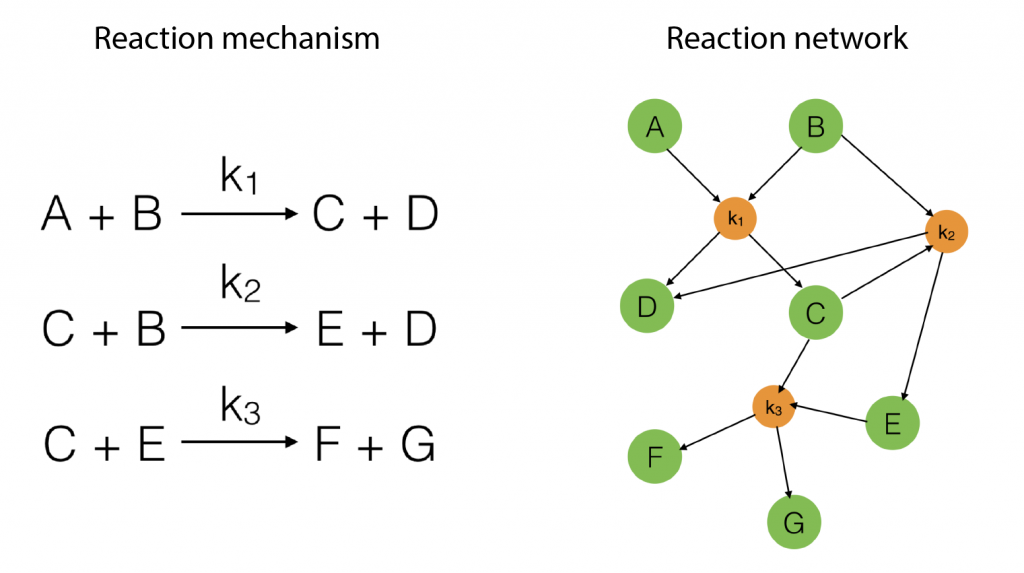
\includegraphics[width=\textwidth]{figs/Graph_example.png}
         \caption{Chemical reactions}
         \label{fig:y equals x}
     \end{subfigure}
     \hfill
     \begin{subfigure}[b]{0.32\textwidth}
         \centering
         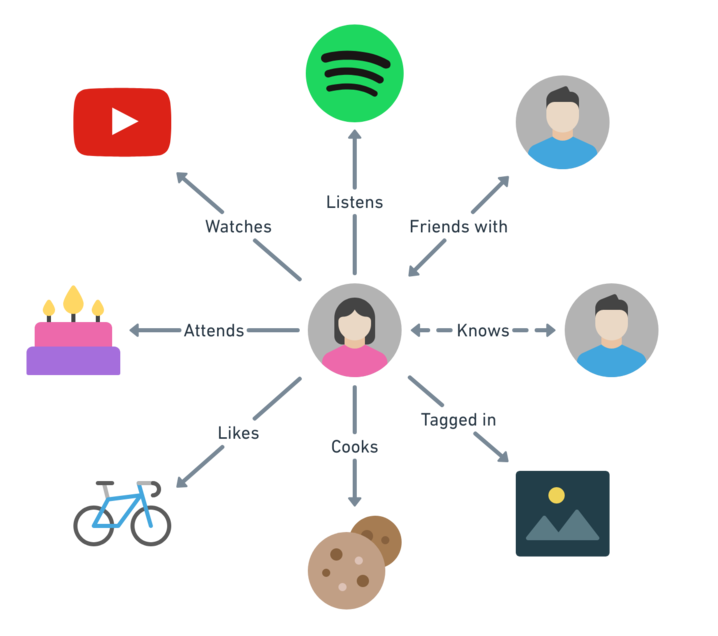
\includegraphics[width=\textwidth]{figs/social_graph_example.png}
         \caption{Social networks}
         \label{fig:three sin x}
     \end{subfigure}
\end{figure}

         \begin{itemize}
        \item  Adjacency matrix to represent a graph of $v$ nodes:
         \begin{itemize}
            \footnotesize
            \item  $\mathbf{A} \in \mathbb{R}^{v\times v}$: $a_{i, j}=1$ if nodes $(i, j)$ have edge, $0$ otherwise.
        \end{itemize}

        \begin{figure}[!htb]
        \centering
        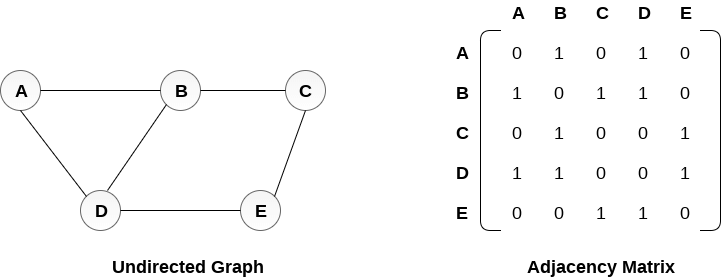
\includegraphics[width=0.5\textwidth]{figs/adjacency matrix.png}
        \end{figure}
    \end{itemize}
\end{frame}


%\subsection{Graph classification}
\begin{frame}{Graph classification \& applications}
\footnotesize
    \begin{itemize}
        \item Supervised classification:
        \begin{itemize}
            \item Pre-labeled  dataset: $(\{\mathcal{G}_1,\ldots,\mathcal{G}_n\}, \{y_1,\ldots,y_n\})$.
            \item Each graph $\mathcal{G}_i$ belongs to class $y_i$.
            \item Task: a classification algorithm that, given in input a new graph, output the class to which it belongs.
        \end{itemize}
        \vfill
        \item  Graphs  have different sizes ($\#$nodes), so a classifier has 2 blocks:
        	\begin{figure}[H]
        	\centering
        	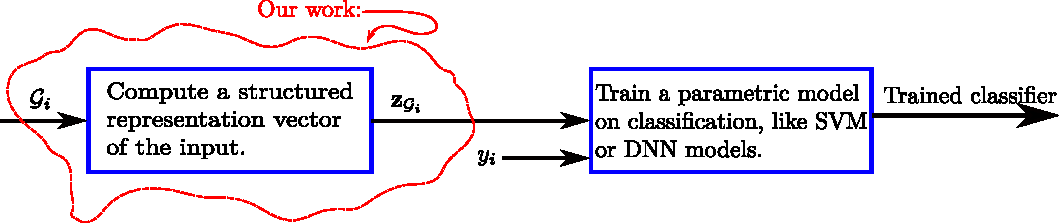
\includegraphics[scale=0.5]{figs/classifier.pdf}
        	\vfill
        \end{figure}

        \vfill 
       \item Applications in real world: Marketing, Banking, Biology.
       \vfill
       \item Example in biology:
       \begin{itemize}
           \item amino acids are linked to form a protein.
           \item enzymes are specific type of proteins 
           \item predict whether a protein is an enzyme or not. 
       \end{itemize}
     \end {itemize}
     
\end{frame}


%\subsection{State-of-the-art methods}
\begin{frame}{State-of-the-art methods}
    
    \begin{itemize} 
    \item Graph kernels based algorithms:
    \begin{itemize}
    \item Fixed graph representation is computed.
    \item \textbf{Graphlet kernel} is based on counting subgraphs.
    \end{itemize}
\end{itemize}
 \vfill
 \textbf{Our Contribution:} inspired by the graphlet kernel, we propose a fast and efficient graph classification framework, which leverages optical random features.
\end{frame}


\begin{frame}{Outline}
\tiny
\tableofcontents
\end{frame}

\section{Background: the graphlet kernel}

\begin{frame}{Necessary tools and definitions}
    \begin{itemize}
    \footnotesize
    \item Graphlet kernel needs an integer parameter $\textcolor{red}{k}$ to be fixed.
    \vfill
      \item Also, the set of all different graphs of size $k$.
          \begin{itemize}
      	\item these graphs are called \textcolor{red}{{\emph{graphlets}}}.
      \end{itemize}
    	\begin{figure}[H]
  	\centering
  	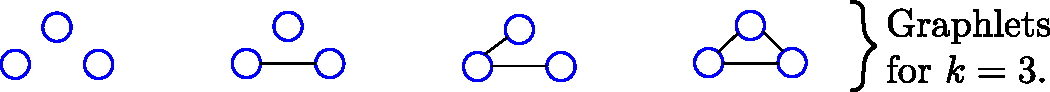
\includegraphics[scale=0.45]{figs/graphlets.pdf}
  	\vfill
  \end{figure}  
	\vfill
  \item Definition: to get a sub-graph $\mathcal{F}$ from a graph $\mathcal{G}$:
  	\begin{figure}[H]
  	\centering
  	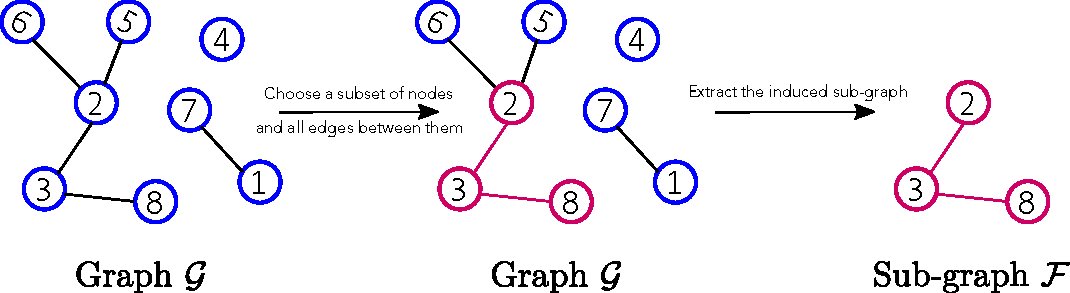
\includegraphics[scale=0.5]{figs/subgraphs.pdf}
  	\vfill
  \end{figure}  

    \end{itemize}
\end{frame}

\begin{frame}{Graphlet kernel illustration}
	\footnotesize
	Goal: compute representation vectors for graphs, for example:
	\begin{figure}[H]
		\centering
		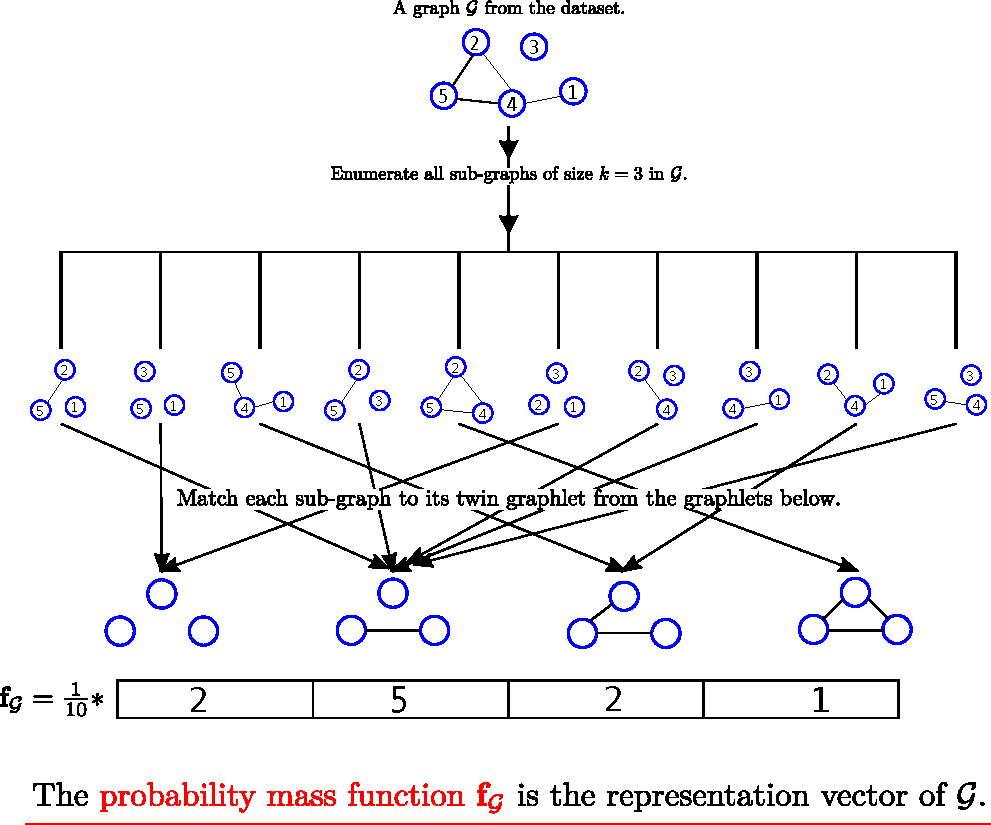
\includegraphics[scale=0.5]{figs/gk.pdf}
		\vfill
	\end{figure}
\end{frame}

\begin{frame}{Graphlet kernel \textbf{cost}}
	\footnotesize
	\begin{figure}[H]
		\centering
		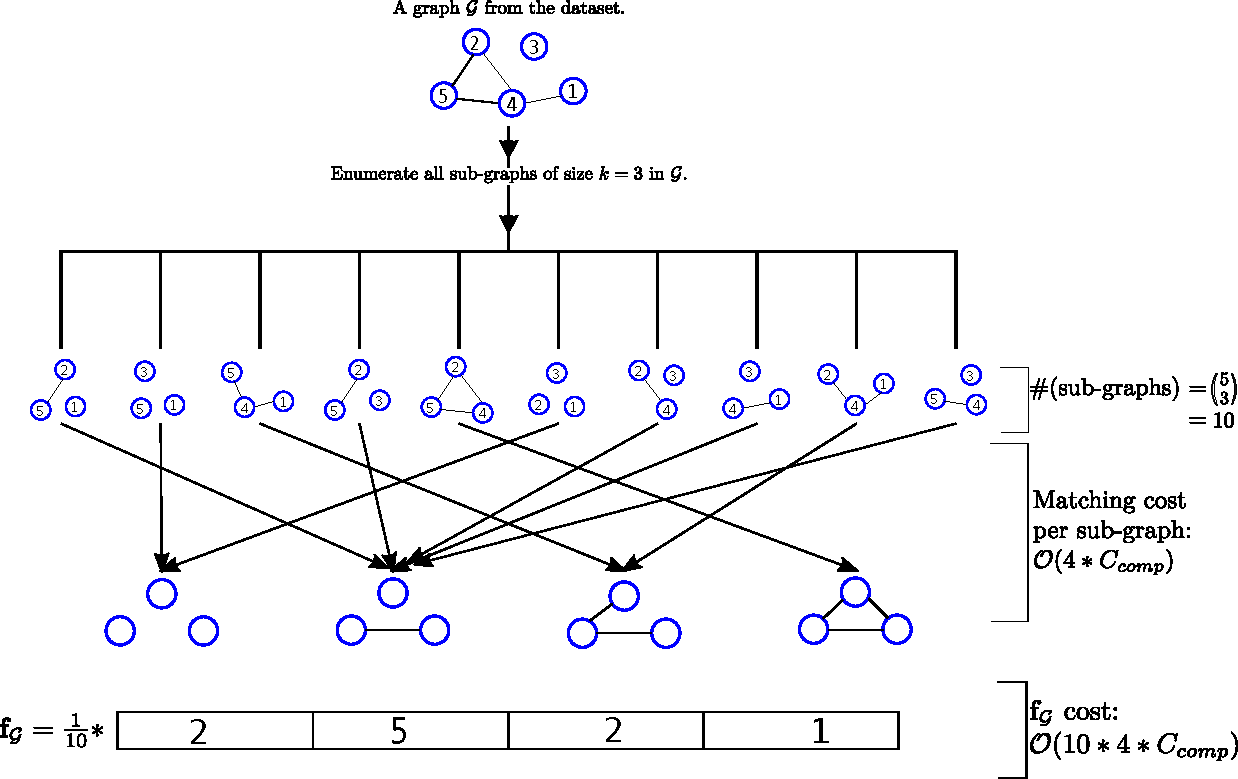
\includegraphics[scale=0.45]{figs/gk_cost.pdf}
		\vfill
	\end{figure}
	$\mathbf{f}_\mathcal{G}$ cost \textcolor{red}{exponential}  in $k$: $C_{gk}=\mathcal{O}(\#subgraphs*\#graphlets*C_{comp})$
\end{frame}

%\begin{frame}{Graphlet kernel \textbf{cost}}
%	\footnotesize
%	\begin{figure}[H]
%		\centering
%		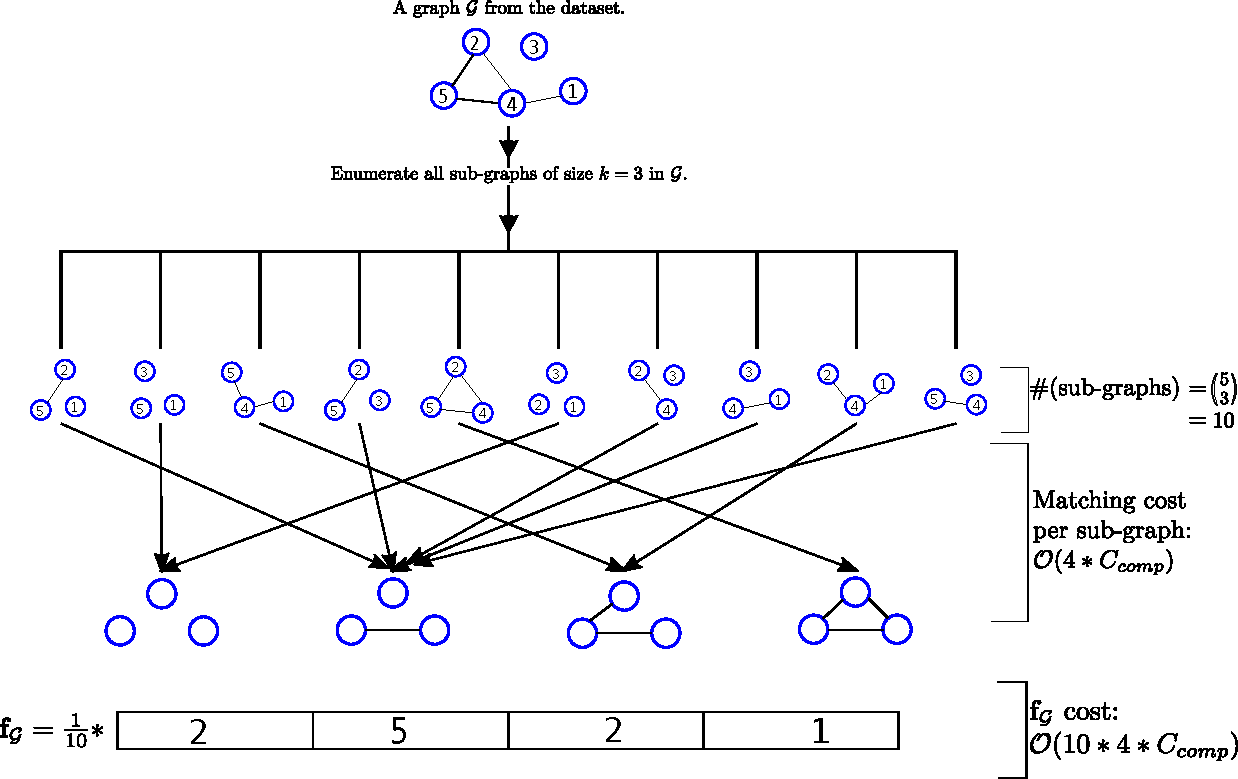
\includegraphics[scale=0.45]{figs/gk_cost.pdf}
%		\vfill
%	\end{figure}
%	But, $\mathbf{f}_\mathcal{G}$  is a \textcolor{red}{probability mass function} on subgraphs in $\mathcal{G}$.
%\end{frame}

\begin{frame}{\textbf{Acceleration}: estimate $\mathbf{f}_\mathcal{G}$ with \textcolor{red}{$s$ subgraphs}}
	\footnotesize
	\begin{figure}[H]
		\centering
		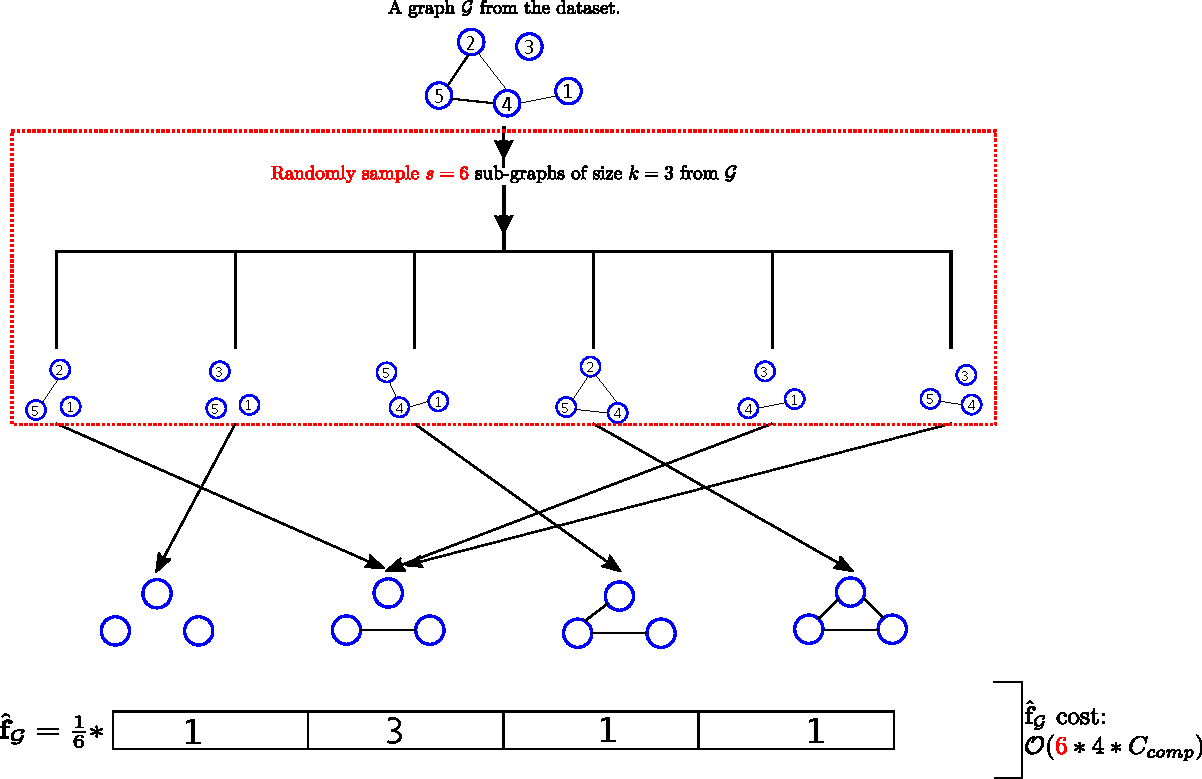
\includegraphics[scale=0.45]{figs/gk_accelerated.pdf}
		\vfill
	\end{figure}
	$\hat{\mathbf{f}}_\mathcal{G}$ cost is lower but still  \textcolor{red}{exponential}  in $k$:
	
	
	{\centering$C_{gk+gs}=\mathcal{O}(s*\#graphlets*C_{comp})$\par}
	
	
	$\Rightarrow$ must deal with the matching stage for a lower cost.
\end{frame}

\begin{frame}{Outline}
	\tiny
	\tableofcontents
\end{frame}

\section{GSA-$\varphi$ algorithm with optical random features}

\begin{frame}{Proposed classification framework $GSA-\varphi$}
	\footnotesize
	Replace subgraph-to-graphlet matching with a fast  user-defined map:
	\vfill
	{\centering $\varphi:$ \{size-$k$ subgraphs\}$\mapsto\mathbb{R}^{\textcolor{red}{m}}\enspace, {\textcolor{red}{m}}$ is user-chosen. \par}
	\begin{figure}[H]
		\centering
		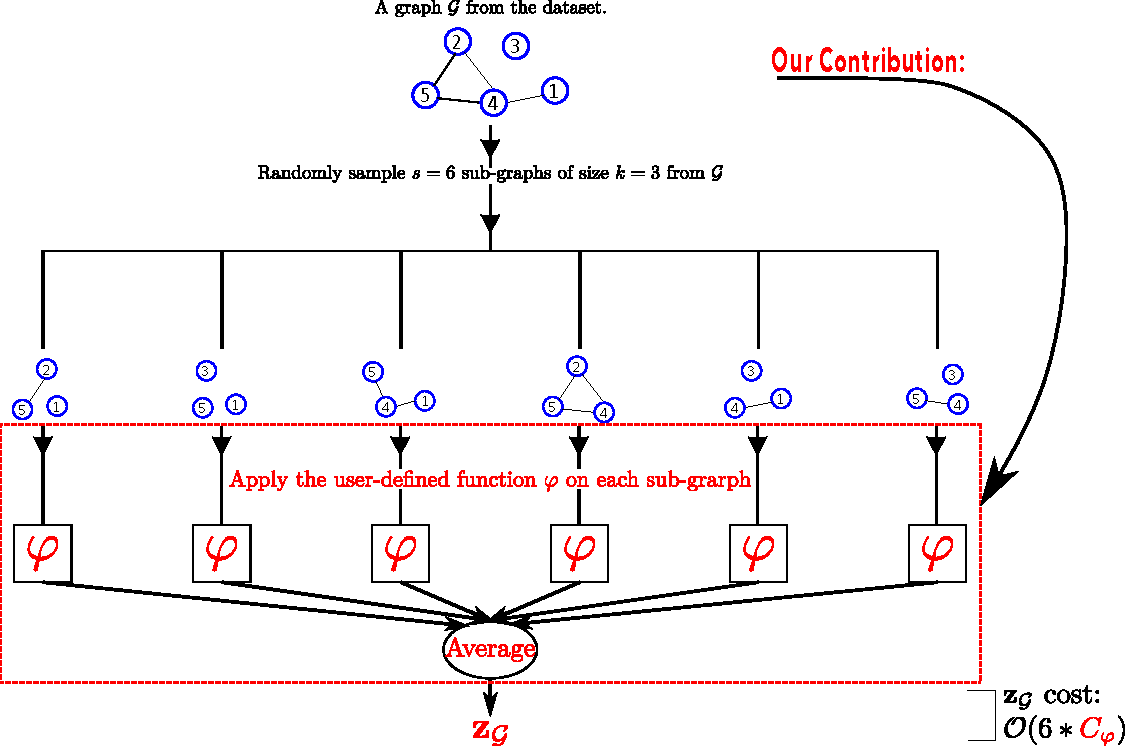
\includegraphics[scale=0.45]{figs/GSA_phi.pdf}
		\vfill
	\end{figure}
	${\mathbf{z}}_\mathcal{G}$ is the representation vector of $\mathcal{G}$, with cost: $C_{GSA-\varphi}=\mathcal{O}(s*C_{\varphi})$.
	
\end{frame}



%\subsection{$GSA-\varphi$ with random features}
%\begin{frame}{$GSA-\varphi$ with kernel random features}
% \begin{itemize}
%    \footnotesize
%        \item $\kappa:\mathcal{D}\times\mathcal{D}\mapsto\mathbb{R}$  is  a positive semi-definite kernel if:
%\begin{center}
%$\forall n\in \mathbb{N},~\forall \alpha\in \mathbb{R}^n,~\forall x_1,\ldots,x_n\in \mathcal{D},\quad \sum_{i,j}^n\alpha_i\alpha_j\kappa(x_i,x_j)\geq 0$ 
%\end{center}
%\vfill
%\item Example: Gaussian kernel
%\begin{center}
%    $\kappa_{G}(\mathbf{x},\mathbf{x}')=\exp^{-\frac{\left \| \mathbf{x}-\mathbf{x}'\right\|^2}{2\sigma^2}}$
%\end{center} 
%        \vfill
%    \end{itemize}
%\end{frame}




\begin{frame}{$GSA-\varphi$ with kernel random features}
    \begin{itemize}
    \footnotesize
        \item Kernels with random features are functions that:\\
        \begin{center}
            $\kappa(\mathbf{x},\mathbf{x}')= \mathbb{E}_{\mathbf{w} \sim p}~ \xi_\mathbf{w}(\mathbf{x})^* \xi_\mathbf{w}(\mathbf{x}')$
        \end{center}

        \vfill
        \item Defining : $\varphi_{RF}(\mathbf{x}) = \frac{1}{\sqrt{m}} ( \xi_{\mathbf{W}_j}(\mathbf{x}) )_{j=1}^m$\\ we can write: $\kappa(\mathbf{x},\mathbf{x}')\approx \varphi_{RF}(\mathbf{x})^*\varphi_{RF}(\mathbf{x}')$
        \vfill
        \item Example: Gaussian kernel $\kappa_{G}(\mathbf{x},\mathbf{x}')=\exp^{-\frac{\left \| \mathbf{x}-\mathbf{x}'\right\|^2}{2\sigma^2}}$ corresponds to:\\
        \begin{center}
            $\varphi(\mathbf{x}) = \frac{\sqrt{2}}{\sqrt{m}} cos( \mathbf{W}^T\mathbf{x}+b ),~ \mathbf{x}\in\mathbb{R}^d,  \mathbf{W}\in \mathbb{R}^{m\times d}$
        \end{center}
        \vfill
        \item $\mathbf{x}$ is a subgraph adjacency matrix $\Rightarrow$ $\varphi_{RF}(\mathbf{x})$ costs: $\mathcal{O}(mk^2)$
        \vfill
        \item  Computation cost of $GSA-\varphi_{RF}=  \mathcal{O}( s m k^2)$
    
\end{itemize}
\end{frame}


\begin{frame}{Concentration analysis}
    \footnotesize
    \begin{itemize}
 \item Recall: ($\mathcal{G} +$ subgraph sampling) $\rightarrow \mathbf{f}_\mathcal{G}$: discrete prob. dist. of graphlets.
    \vfill
  \item Recall: $\mathbf{z}_\mathcal{G}$ is the graph representation of $GSA-\varphi$.
  \vfill
        \item The Euclidean metric $\|\mathbf{z}_\mathcal{G} - \mathbf{z}_{\mathcal{G}'}\|^2$ converges to the \textbf{MMD metric}:    $MMD(\mathbf{f}_\mathcal{G},\mathbf{f}_{\mathcal{G}'})^2$\\
%            \begin{center}
%            $MMD(f_\mathcal{G},f_{\mathcal{G}'})^2 = \mathbb{E}_{\mathbf{w}} \Big( \left| \mathbb{E}_{F\sim f_\mathcal{G}} \xi_\mathbf{w}(F) - \mathbb{E}_{F'\sim f_{\mathcal{G}'}} \xi_\mathbf{w}(F') \right|^2 \Big)$    
%        \end{center}
        \item MMD is a true metric on distributions for many schemes of kernel random features
    \end{itemize}
    \vfill
    \begin{theorem}
Let $\mathcal{G}$ and $\mathcal{G}'$ be two graphs.  Assume that $|\xi_\mathbf{w}(F)| \leq 1$.

Then, for all $\delta>0$, with probability at least $1-\delta$:
\begin{align*}
 \Big|\| \mathbf{z}_\mathcal{G} - \mathbf{z}_{\mathcal{G}'}\|^2 - MMD(\mathbf{f}_\mathcal{G},\mathbf{f}_{\mathcal{G}'})^2 \Big| \leq \\\frac{4 \sqrt{\log (6/\delta)}}{\sqrt{m}} + \frac{8\left(1+\sqrt{2\log(3/\delta)}\right)}{\sqrt{{s}}}
\end{align*}
\end{theorem}
\end{frame}




%\subsection{$GSA-\varphi$ with optical random features}
\begin{frame}{$GSA-\varphi$ with optical random features}
    \begin{itemize}
    \footnotesize
        \item Model: $\mathbf{\varphi}_{OPU}(\mathbf{x})=|\mathbf{Wx+b}|^2 ;~\mathbf{W}\in \mathbb{R}^{m\times d},\mathbf{b}\in \mathbb{R}^m, \mathbf{x}\in \mathbb{R}^d$
        \item When $m\mapsto\infty$ then: $\mathbf{\varphi}_{OPU}(\mathbf{x_1})^T\mathbf{\varphi}_{OPU}(\mathbf{x_2})\approx \kappa_{OPU}(\mathbf{x_1}, \mathbf{x_2})$
    \end{itemize}
    \begin{figure}[ht!]
\begin{center}
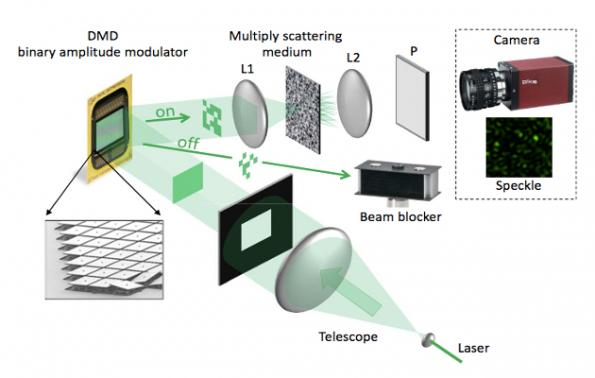
\includegraphics[scale=0.3]{figs/lighton630.jpg}
\end{center}
\caption*{OPU's Experimental setup \citep{saade2016random}.}
\label{fig_opu}
\end{figure}
\begin{itemize}
    \item $C_{\varphi_{OPU}}=\mathcal{O}(1)$ in the input and output dimensions.
    \vfill
          \item The computation cost  $C_{GSA-\varphi_{OPU}} =   \mathcal{O}(s)$

\end{itemize}
\end{frame}

\begin{frame}{Comparison between computation costs}
\begin{table}
	\centering
	\begin{tabular}{|c|c|c|}
		\hline
		\multicolumn{2}{|c|}{Graphlet kernel} & $O\big(s* (\#graphlets)*C_{comp}\big)$\\ \hline \hline
		%
		\multirow{3}{*}{GSA-$\varphi$ with:} & 
		 $\varphi_{Gs}$ & $O(s m k^2)$ \\ 
		& $\varphi_{Gs+eig}$  & $O(s (m k + k^3))$ \\ 
		& $\varphi_{OPU}$  & $O( s)$ \\ \hline
	\end{tabular}
	\label{tab:cost}
	~\vspace{-0.8cm}
\end{table}%
%\caption{Complexities of the different mappings used in GSA-$\varphi$.}
\end{frame}

\begin{frame}{Outline}
\tiny
\tableofcontents
\end{frame}



\section{Results and Discussion}

%\subsection{Compare difference choices of $\varphi$}
%\begin{frame}{Compare difference choices of $\varphi$}
%\footnotesize
%\begin{itemize}
%    \item Dataset: 
%    \begin{itemize}
%        \item 300 2-classes labeled graphs
%        \item generated based on SBM model
%        \item  inter-class similarity parameter $r$ controls the problem difficulty.
%    \end{itemize}
%\end{itemize}
% \begin{figure}[h]
%\centering
%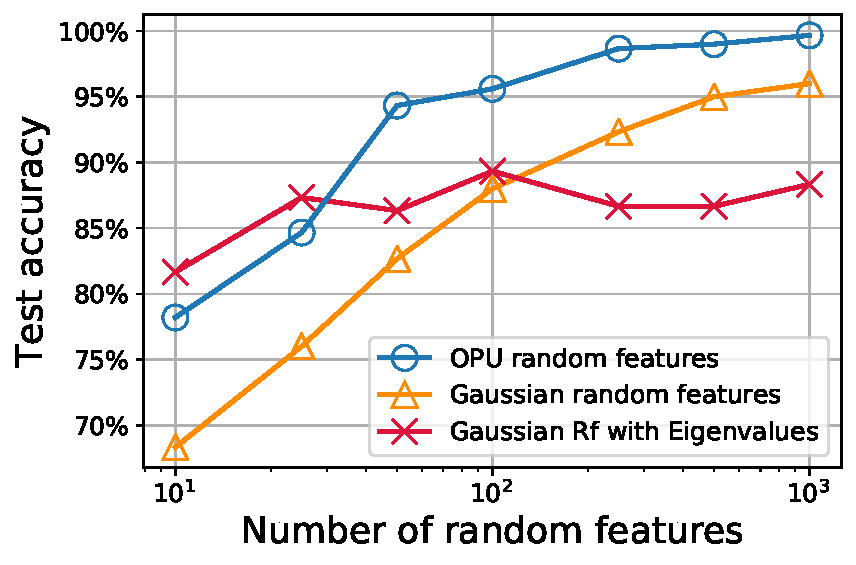
\includegraphics[scale=0.4]{figs/phi_comparison.pdf}
%
%\centering 
%{Comparing different $\varphi_{RF}$ maps in $GSA-\varphi$. 
%	
%	Fixed parameters: $r=1.1$, $k=6$,  $s=2000$, and $\sigma=0.1$.}
%%Source:
%\label{fig:phi_comparison}
%\end{figure}
%\end{frame}

%\subsection{$GSA-\varphi_{OPU}$ Vs. graphlet kernel}
\begin{frame}{$GSA-\varphi_{OPU}$ Vs.  graphlet kernel and GCN models}
\footnotesize
\begin {itemize}
    \item Dataset: 
\begin{itemize}
	\item 300 2-classes labeled graphs.
	\item generated based on SBM model.
	\item  inter-class similarity  $r$ controls the problem difficulty.
\end{itemize}
\end {itemize}
\vfill
 \begin{figure}[h]
\centering
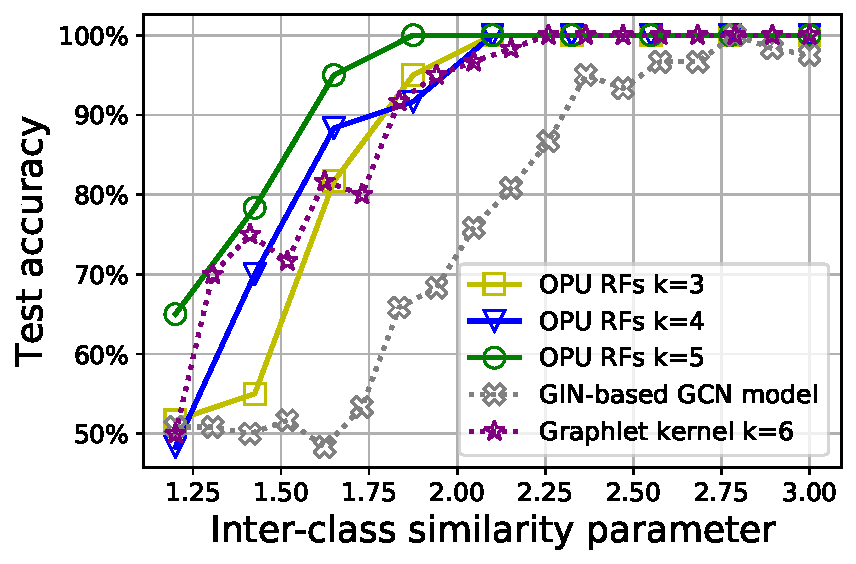
\includegraphics[scale=0.4]{figs/gk_vs_opu.pdf}
\end{figure}

\centering { Fixed parameters: $s=2000$, $m=5000$}
\end{frame}

\begin{frame}{$k$-graphlet Kernel for $k=3$}
\footnotesize
\begin{figure}[H]
\centering
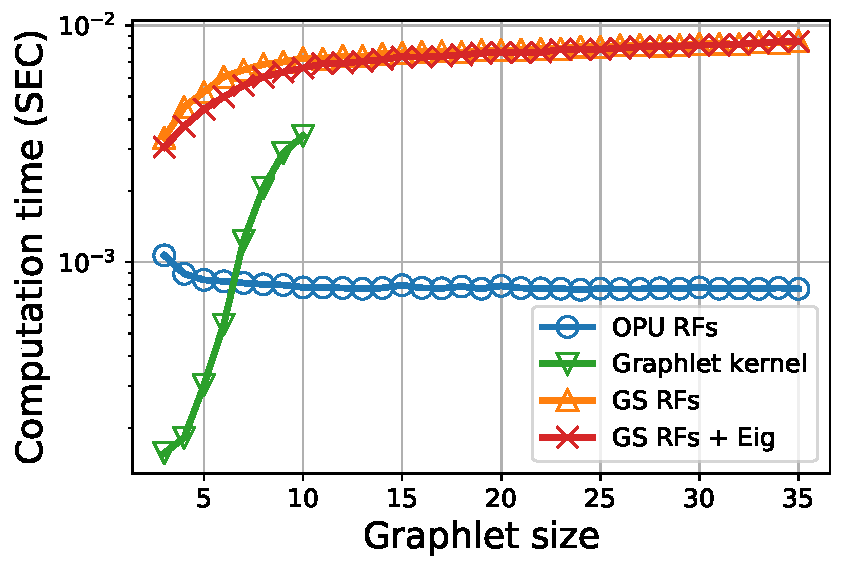
\includegraphics[scale=0.4]{figs/computational_comp.pdf}
\vfill
\centering  Fixed parameters: $r=1.1$,  $s=2000$, $m=5000$ and  $\sigma =0.1$.
\end{figure}
\end{frame}



%\begin{frame}{Uniform sampling Vs. random walk sampling}
%	\begin {itemize}
%		\item GSA-$\varphi_{OPU}$ with different graph sampling techniques, and different values of the graphlet size $k$.
%	\end {itemize}
%\begin{figure}
%     \centering
%     \begin{subfigure}[b]{0.49\textwidth}
%         \centering
%         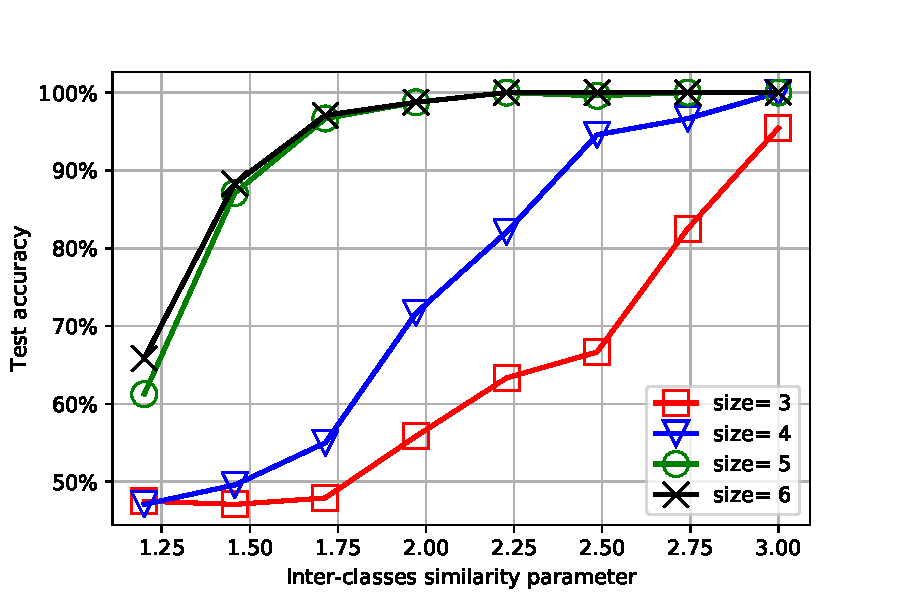
\includegraphics[width=\textwidth]{figs/LightOn_adj_SBM_Similarity_graphlet_size.pdf}
%         \caption{Uniform sampling}
%         \label{fig:y equals x}
%     \end{subfigure}
%     \hfill
%     \begin{subfigure}[b]{0.49\textwidth}
%         \centering
%         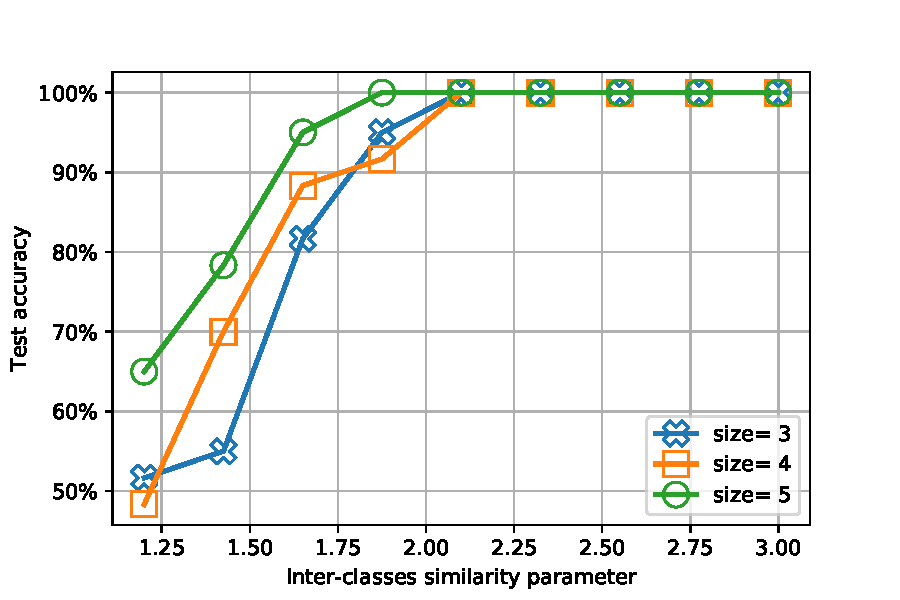
\includegraphics[width=\textwidth]{figs/LightOn_adj_SBM_similarity_graphlet_size_RW.pdf}
%         \caption{Random Walk sampling}
%         \label{fig:three sin x}
%     \end{subfigure}
%\end{figure}
%\end{frame}


\begin{frame}{$GSA-\varphi_{OPU}$ on the Reddit dataset }
	\begin{itemize}
		\item $k=7$, $s=4000$. 
		\item For every $m$, the experiment is repeated 4 times (red dots), then  averaged (blue curve).
	\end{itemize}
\begin{figure}[H]
\centering
\includegraphics[scale=0.4]{figs/reddit.pdf}
\end{figure}
\end{frame}

\begin{frame}{Conclusion and future work }
\footnotesize
\textbf{Conclusion:}
\begin{enumerate}
    \item GSA-$\varphi$ with RF maps separates well between graphs. 
    \item GSA-$\varphi$ with optical RF maps is  faster than traditional graphlet kernel.
    \item GSA-$\varphi$ with optical RF maps performs better than the graphlet kernel, and better than a particular graph convolutional networks on graph classification.
\end{enumerate}
\vfill
\textbf{Future work:}
\begin{enumerate}
    \item  Combine our algorithm with GCNs when we have node features.
    \item Further analysis of the MMD metric properties on particular graph models. 
\end{enumerate}

\end{frame}{}

%\begin{frame}
%\begin{center}
%\textbf{Thank you for listening}    
%\end{center}
%\end{frame}

\begin{frame}[allowframebreaks]{References}
	\nocite{*}
	\footnotesize
	\bibliographystyle{unsrtnat}
	\bibliography{refs.bib} % file name of the bibtex
\end{frame}

\end{document}

